\subsection*{Problema 18}
\textbf{Enunciado:} Calcular la integral:
\begin{equation*}
\int \frac{\sin x \, dx}{\cos^2 x - \cos x - 2}
\end{equation*}

\textbf{Solución:} Para resolver la integral dada, 
aplicamos el cambio de variable sugerido 
$u = \cos x$, de donde obtenemos 
$du = -\sin x \, dx$, o bien, 
$\sin x \, dx = -du$.

Sustituyendo en la integral original, 
obtenemos:
\begin{align*}
\int \frac{\sin x \, dx}{\cos^2 x - \cos x - 2} 
&= \int \frac{-du}{u^2 - u - 2} \\
&= -\int \frac{du}{u^2 - u - 2}
\end{align*}

Factorizamos el denominador utilizando las 
indicaciones provistas:
\begin{equation*}
u^2 - u - 2 = (u - 2)(u + 1)
\end{equation*}

Planteamos la descomposición en fracciones 
parciales para el integrando:
\begin{align*}
\frac{1}{(u - 2)(u + 1)} 
&= \frac{A}{u - 2} + \frac{B}{u + 1}
\end{align*}

Multiplicando por el denominador común, 
encontramos los coeficientes $A$ y $B$:
\begin{equation*}
1 = A(u + 1) + B(u - 2)
\end{equation*}

Si $u = 2$, se tiene $1 = A(3) \implies A = \dfrac{1}{3}$.
Si $u = -1$, se tiene $1 = B(-3) \implies B = -\dfrac{1}{3}$.

Reemplazando las fracciones parciales en 
la integral:
\begin{align*}
-\int &\left( \frac{1/3}{u - 2} - \frac{1/3}{u + 1} \right) du \\
&= -\frac{1}{3} \int \frac{du}{u - 2} 
+ \frac{1}{3} \int \frac{du}{u + 1}
\end{align*}

Integramos cada término aplicando logaritmos:
\begin{align*}
&= -\frac{1}{3} \ln|u - 2| + \frac{1}{3} \ln|u + 1| + C \\
&= \frac{1}{3} \ln\left| \frac{u + 1}{u - 2} \right| + C
\end{align*}

Finalmente, regresamos a la variable original 
mediante la sustitución $u = \cos x$:
\begin{equation*}
\int \frac{\sin x \, dx}{\cos^2 x - \cos x - 2} 
= \frac{1}{3} \ln\left| \frac{\cos x + 1}{\cos x - 2} \right| + C
\end{equation*}

\begin{figure}[H]
	\centering
	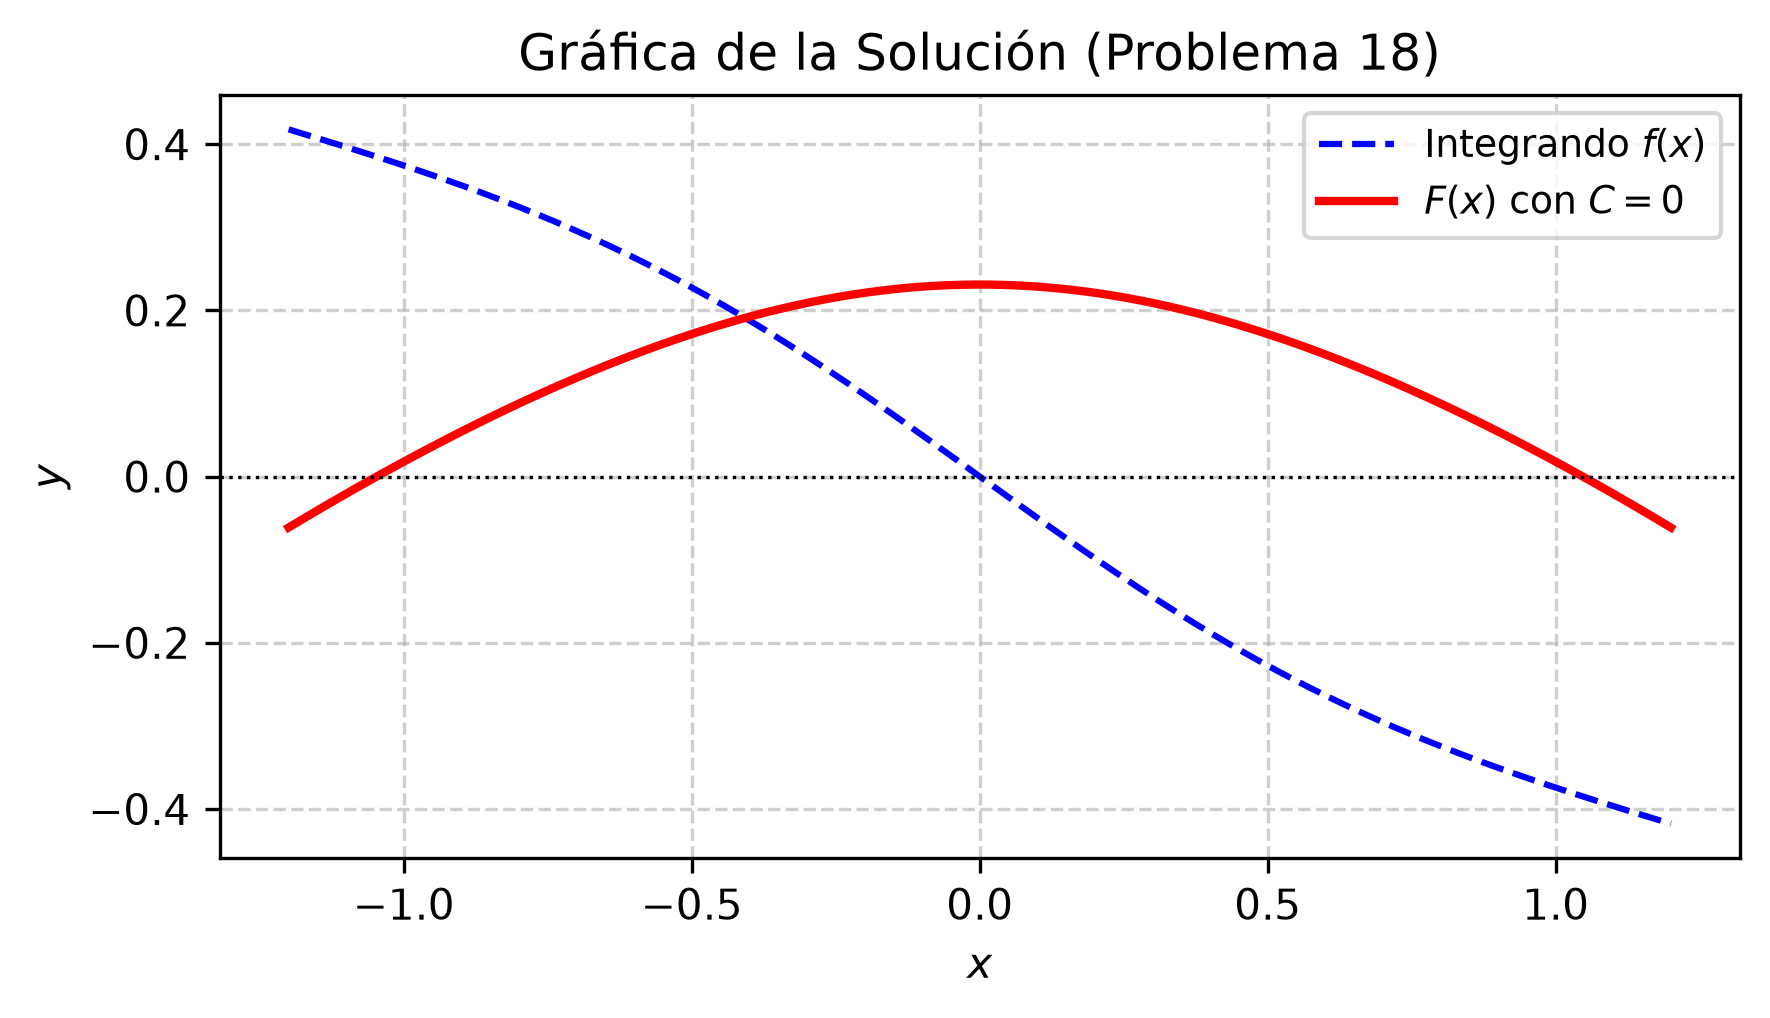
\includegraphics[width=\columnwidth]{semana_04/graficas/SEM04_P18_grafica.png}
	\caption{Representación gráfica de $f(x)$ y su antiderivada $F(x)$ evaluada para la constante de integración $C = 0$ (Problema 18).}
	\label{fig:problema18}
\end{figure}
